\documentclass{sigchi-ext}
% Please be sure that you have the dependencies (i.e., additional
% LaTeX packages) to compile this example.
\usepackage[T1]{fontenc}
\usepackage{textcomp}
\usepackage[scaled=.92]{helvet} % for proper fonts
\usepackage{graphicx} % for EPS use the graphics package instead
\usepackage{balance}  % for useful for balancing the last columns
\usepackage{booktabs} % for pretty table rules
\usepackage{ccicons}  % for Creative Commons citation icons
\usepackage{ragged2e} % for tighter hyphenation
\usepackage{subcaption}

% Some optional stuff you might like/need.
% \usepackage{marginnote} 
% \usepackage[shortlabels]{enumitem}
% \usepackage{paralist}
% \usepackage[utf8]{inputenc} % for a UTF8 editor only

%% EXAMPLE BEGIN -- HOW TO OVERRIDE THE DEFAULT COPYRIGHT STRIP --
% \copyrightinfo{Permission to make digital or hard copies of all or
% part of this work for personal or classroom use is granted without
% fee provided that copies are not made or distributed for profit or
% commercial advantage and that copies bear this notice and the full
% citation on the first page. Copyrights for components of this work
% owned by others than ACM must be honored. Abstracting with credit is
% permitted. To copy otherwise, or republish, to post on servers or to
% redistribute to lists, requires prior specific permission and/or a
% fee. Request permissions from permissions@acm.org.\\
% {\emph{CHI'14}}, April 26--May 1, 2014, Toronto, Canada. \\
% Copyright \copyright~2014 ACM ISBN/14/04...\$15.00. \\
% DOI string from ACM form confirmation}
%% EXAMPLE END

% Paper metadata (use plain text, for PDF inclusion and later
% re-using, if desired).  Use \emtpyauthor when submitting for review
% so you remain anonymous.
\def\plaintitle{SIGCHI Extended Abstracts Sample File: Note Initial
  Caps} \def\plainauthor{First Author, Second Author, Third Author}
\def\emptyauthor{}
\def\plainkeywords{Machine Learning; Codeblocks Programming; Novice Programmer Practices; Interactive Machine Learning}
\def\plaingeneralterms{Programming}

\title{TREX: A Visualization Tool For Linear Regression Experiments To Help Novice Programmers}

\numberofauthors{6}
% Notice how author names are alternately typesetted to appear ordered
% in 2-column format; i.e., the first 4 autors on the first column and
% the other 4 auhors on the second column. Actually, it's up to you to
% strictly adhere to this author notation.
\author{%
  \alignauthor{%
    \textbf{Jordan Aiko Deja}\\
    \affaddr{De La Salle University} \\
    \affaddr{Manila, Philippines} \\
    \affaddr{University of Primorska} \\
    \affaddr{Koper, Slovenia} \\
    \affaddr{jordan.deja@dlsu.edu.ph} }
  \alignauthor{%
    \textbf{Jose Maria Santiago III}\\
    \affaddr{De La Salle University}\\
    \affaddr{Manila, Philippines} \\
    \email{jose\_maria\_santiago@dlsu.edu.ph} } \vfil 
  \alignauthor{%
    \textbf{Giselle Nodalo}\\
    \affaddr{De La Salle University}\\
    \affaddr{Manila, Philippines} \\
    \email{giselle\_nodalo@dlsu.edu.ph} }
  }

% Make sure hyperref comes last of your loaded packages, to give it a
% fighting chance of not being over-written, since its job is to
% redefine many LaTeX commands.
\definecolor{linkColor}{RGB}{6,125,233}
\hypersetup{%
  pdftitle={\plaintitle},
%  pdfauthor={\plainauthor},
  pdfauthor={\emptyauthor},
  pdfkeywords={\plainkeywords},
  bookmarksnumbered,
  pdfstartview={FitH},
  colorlinks,
  citecolor=black,
  filecolor=black,
  linkcolor=black,
  urlcolor=linkColor,
  breaklinks=true,
}

% \reversemarginpar%

\begin{document}



\begin{marginfigure}[3.0pc]
\begin{minipage}{\marginparwidth}
     \centering
    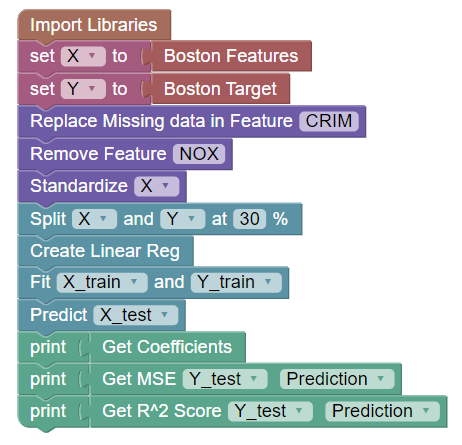
\includegraphics[width=4.5cm,height=4.5cm]{figures/IT3.png}
    \caption{Snippet of the codeblocks of the latest prototype. Codeblocks of the same function are colored and grouped together. }
    \label{fig:IT3_Blocks}
    \end{minipage}
\end{marginfigure}




\begin{marginfigure}[5pc]
\begin{minipage}{\marginparwidth}
     \centering
    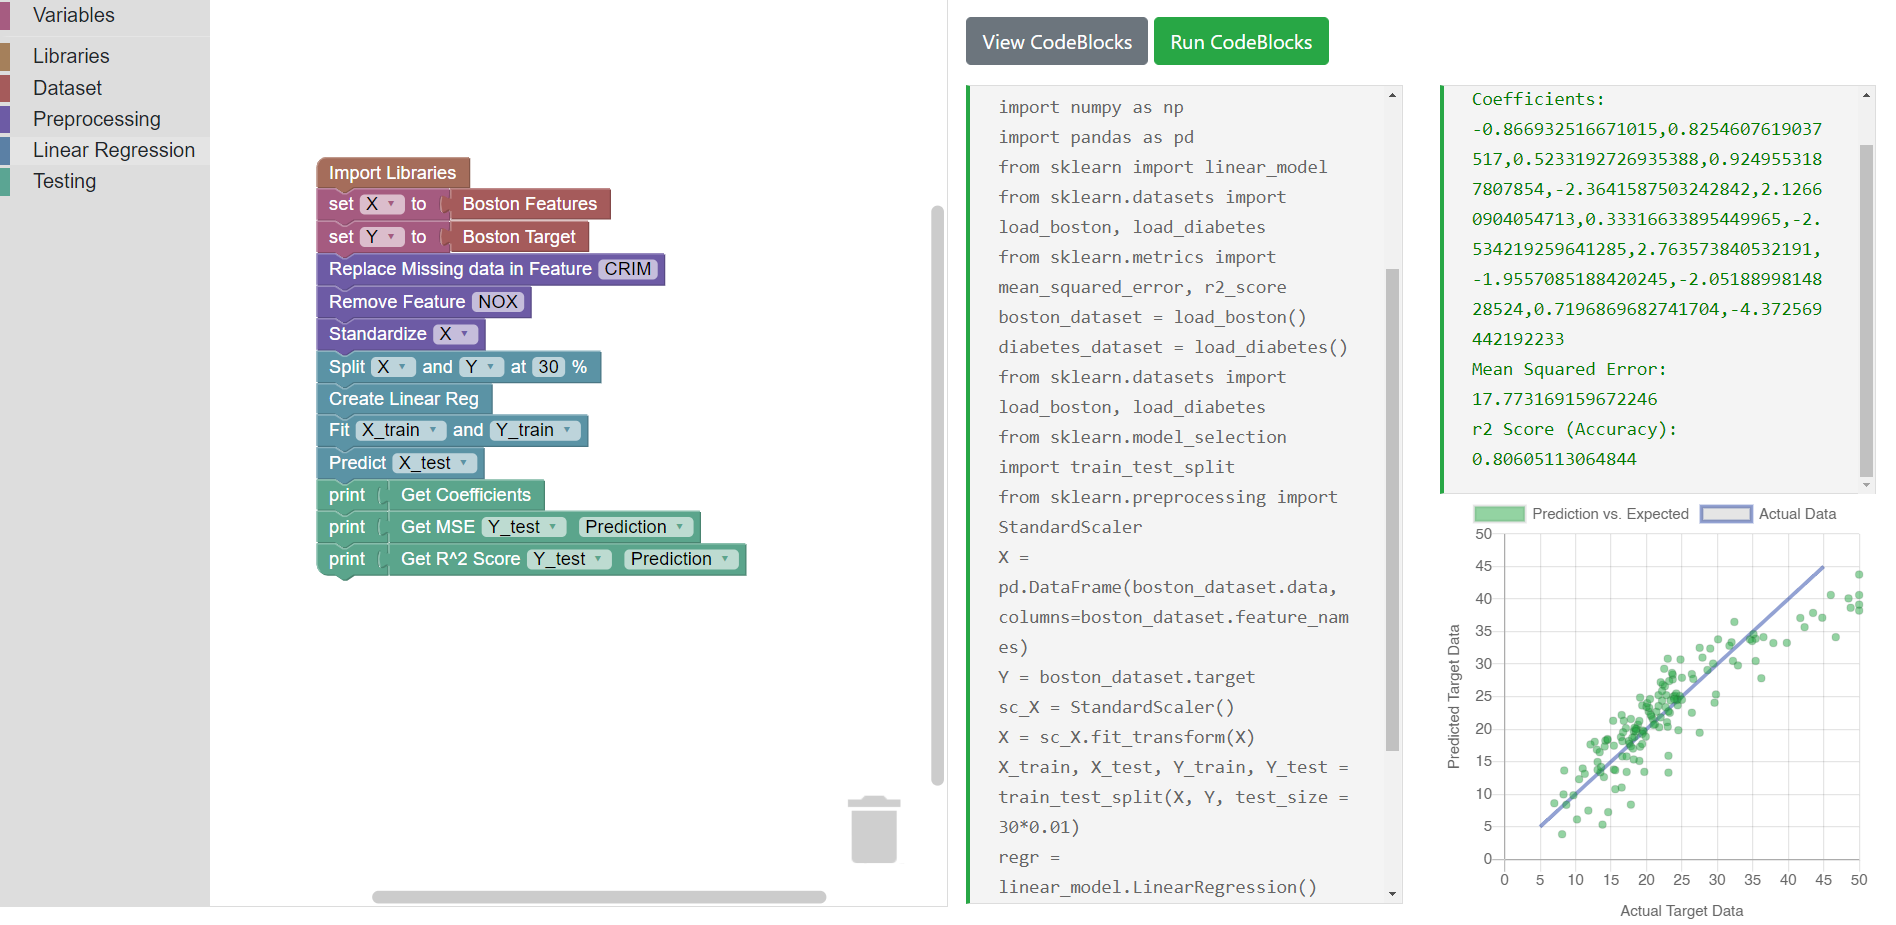
\includegraphics[width=4.75cm,height=3cm]{figures/Gen_Interface.png}
  \caption{A sample screenshot of the third prototype. The leftmost pane has a palette of block groups. The second left pane is a sandbox where they can drag and drop code blocks. The rightmost panes show the equivalent code. }
    \label{fig:prot3}
    \end{minipage}
\end{marginfigure}

%% For the camera ready, use the commands provided by the ACM in the Permission Release Form.
\CopyrightYear{2020}
\setcopyright{rightsretained}
\conferenceinfo{CHI'20,}{April  25--30, 2020, Honolulu, HI, USA}
\isbn{978-1-4503-6819-3/20/04}
\doi{https://doi.org/10.1145/3334480.XXXXXXX}
%% Then override the default copyright message with the \acmcopyright command.
\copyrightinfo{\acmcopyright}


\maketitle

% Uncomment to disable hyphenation (not recommended)
% https://twitter.com/anjirokhan/status/546046683331973120
\RaggedRight{} 

\begin{comment}
\subsection{Iteration 1}
\subsubsection{Prototype Visualizer Design}
\begin{figure}%[ht]
  \centering
    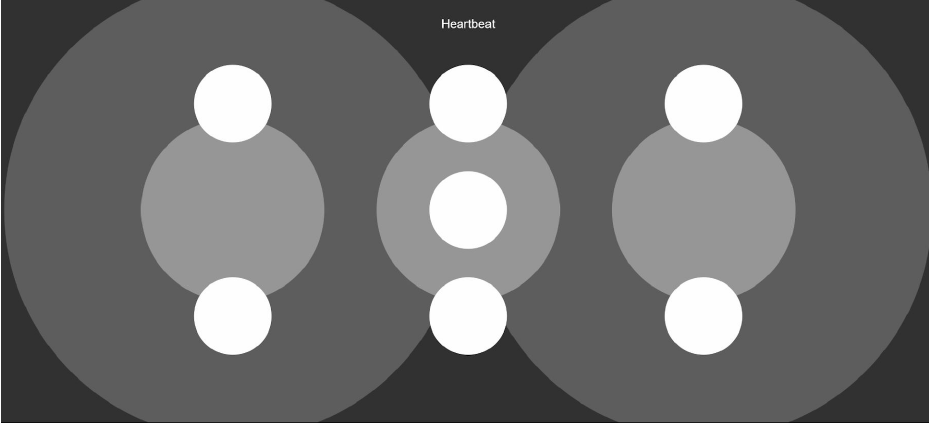
\includegraphics[width=7.5cm,height=4cm]{figures/Prot1.png}
  \caption{A sample screen of the first prototype}
  \label{fig:prot1}
\end{figure}
\subsubsection{Test Design and Experiment Setup}
\begin{figure}%[ht]
  \centering
    \includegraphics[width=7.5cm,height=4cm]{figures/iter1Setup.jpg}
  \caption{Experiment setup for iteration 1}
  \label{fig:iter1Setup}
\end{figure}

\subsection{Iteration 2}
\subsubsection{Prototype Visualizer Design}
\begin{figure}%[ht]
  \centering
    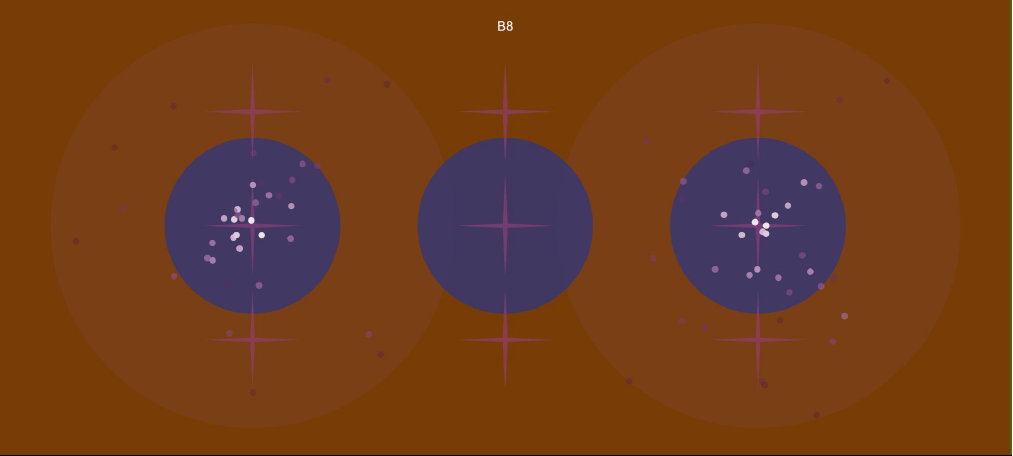
\includegraphics[width=7.5cm,height=4cm]{figures/Prot2.png}
  \caption{A sample screen of the second prototype}
  \label{fig:prot2}
\end{figure}
\subsubsection{Test Design and Experiment Setup}
\begin{figure}%[ht]
  \centering
    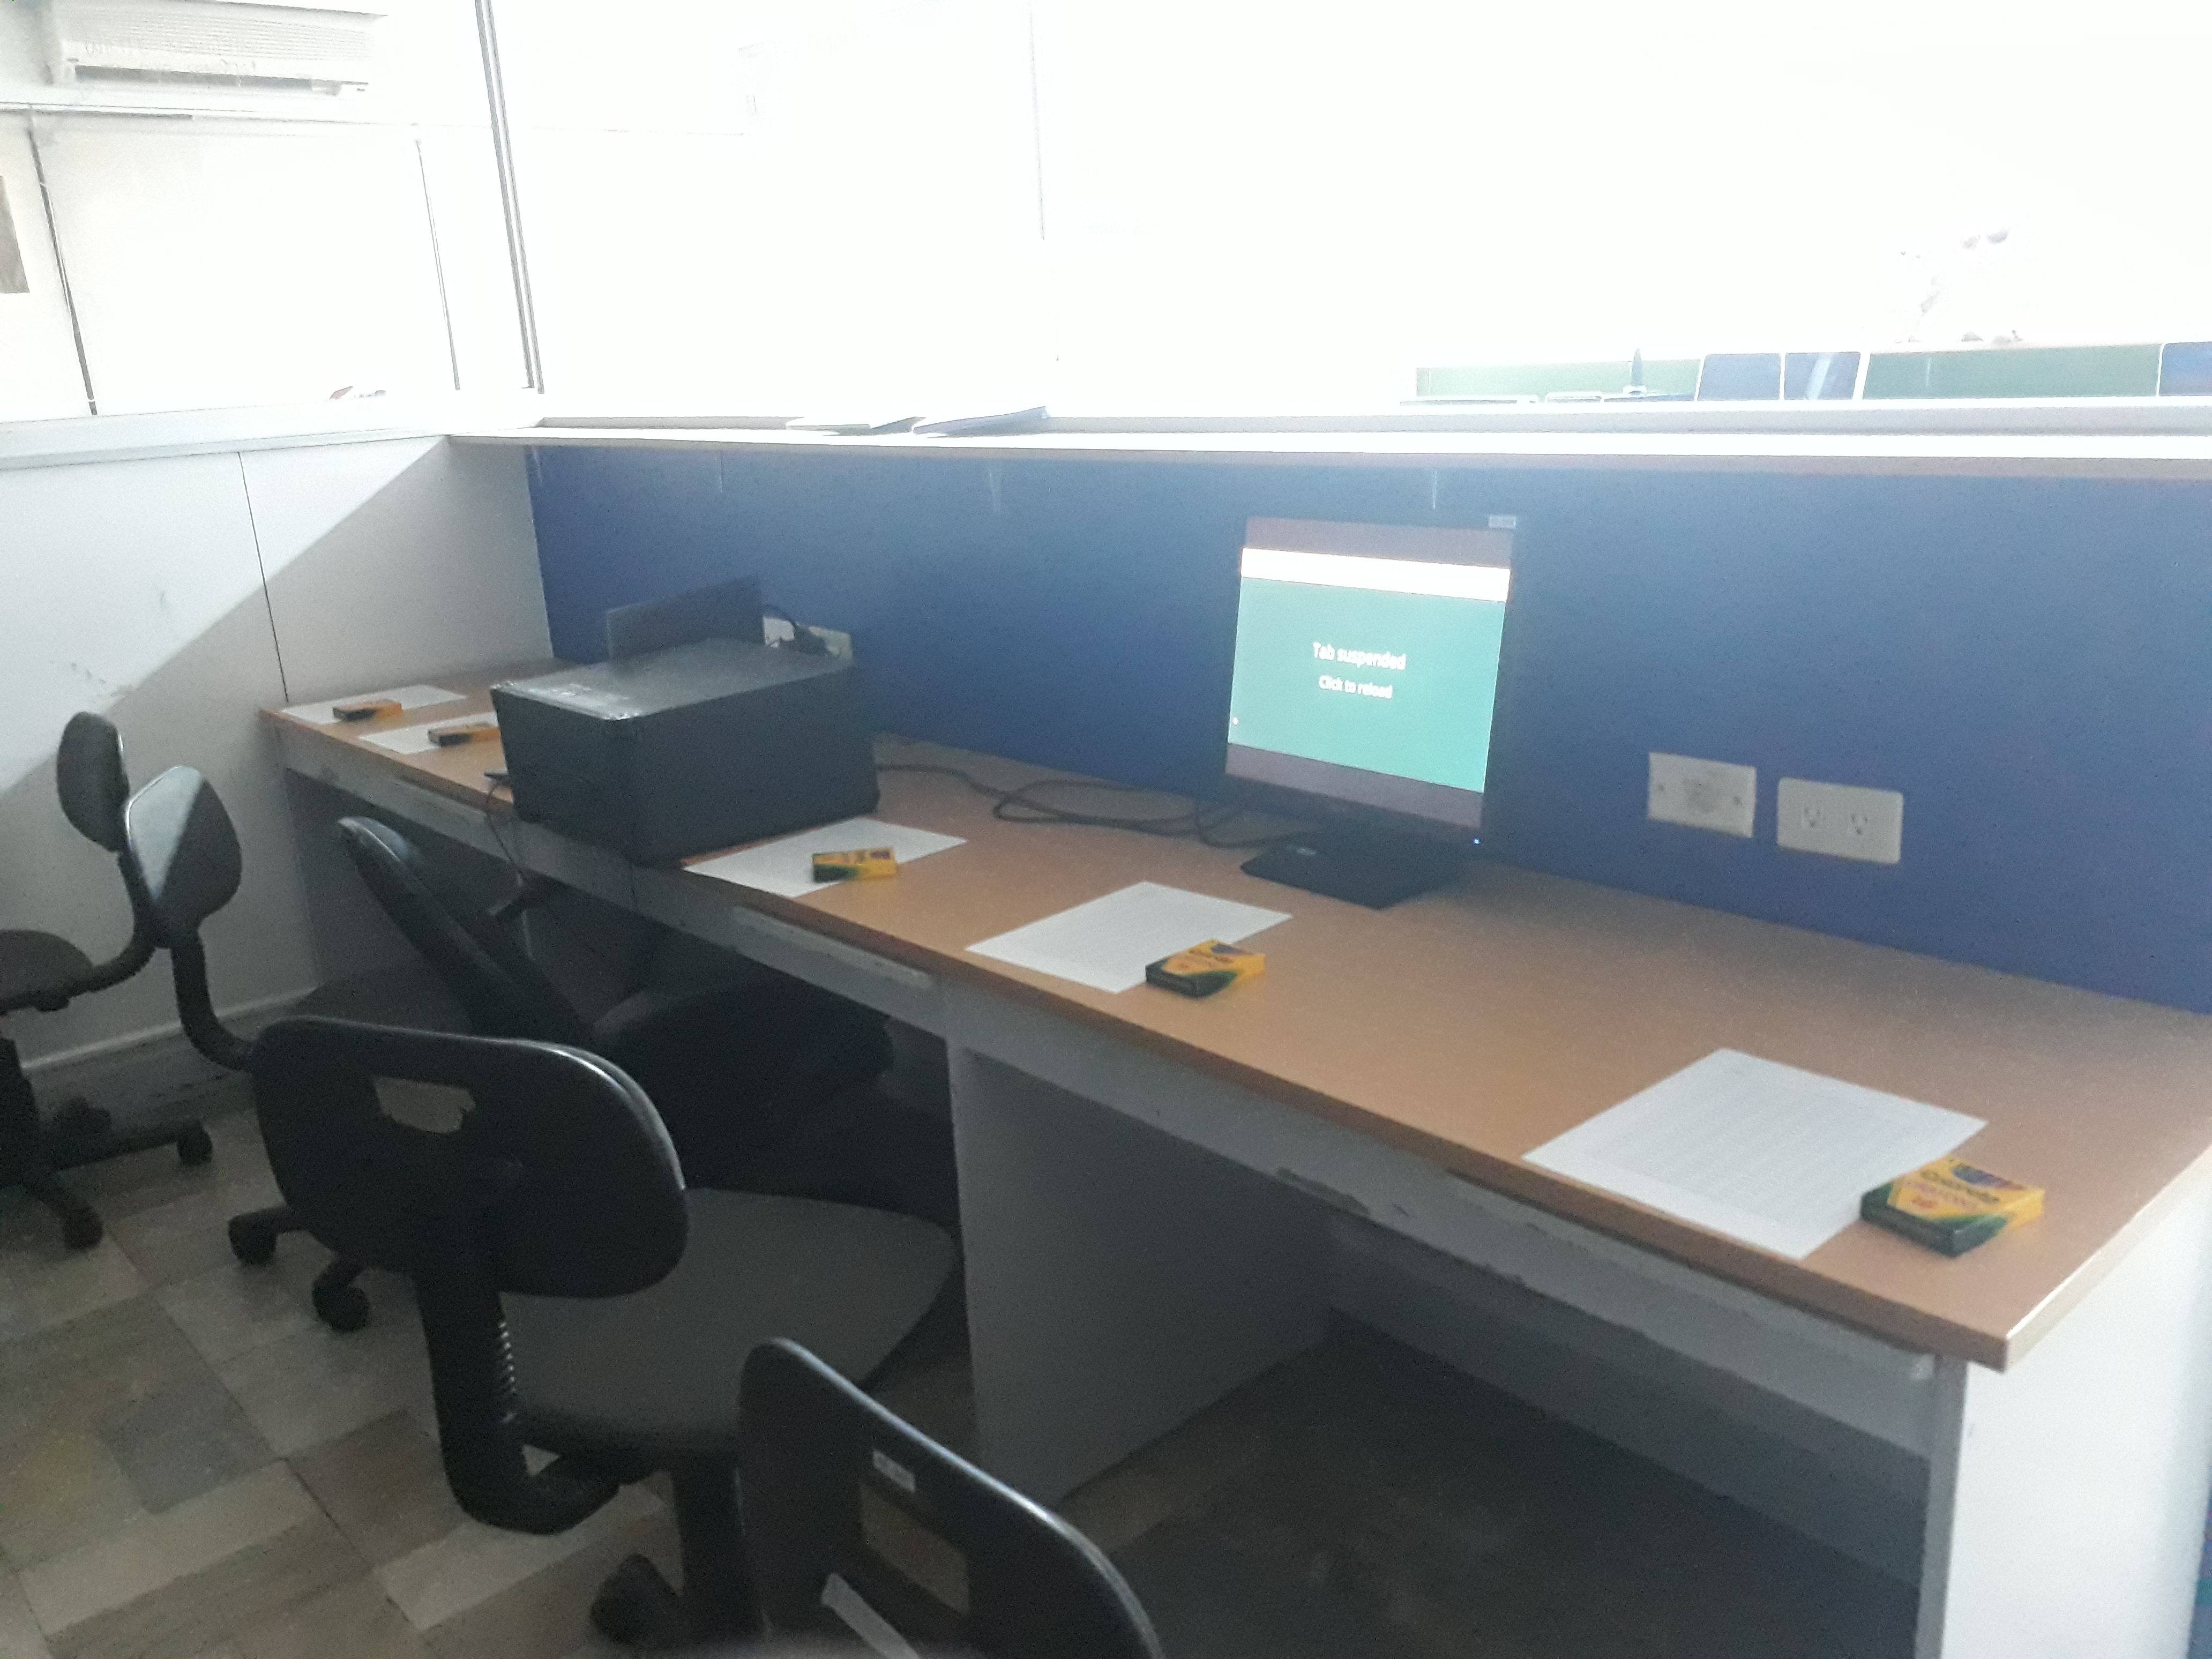
\includegraphics[width=7.5cm,height=4cm]{figures/iter2Setup.jpg}
  \caption{Experiment setup for iteration 2}
  \label{fig:iter2Setup}
\end{figure}

\subsection{Iteration 3}
\begin{figure}%[ht]
  \centering
    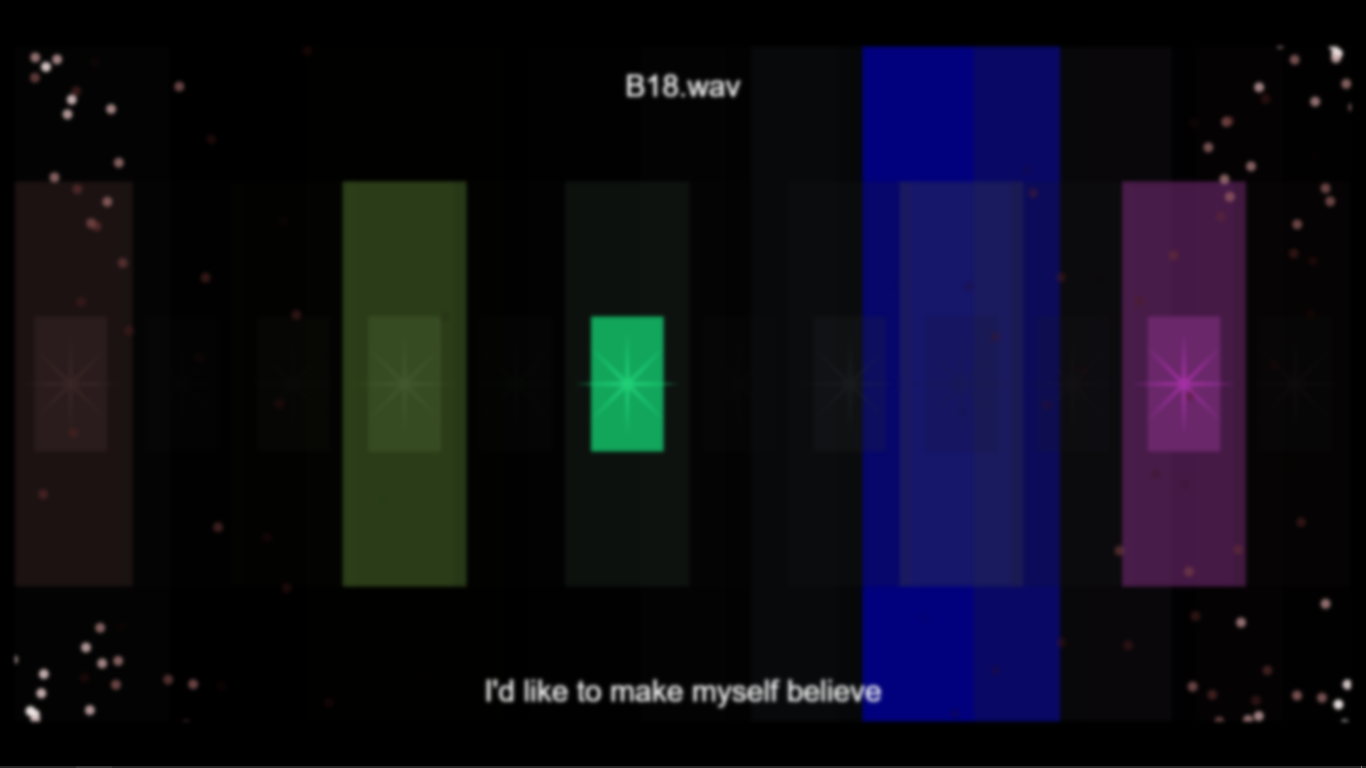
\includegraphics[width=7.5cm,height=4cm]{figures/Prot3.png}
  \caption{A sample screen of the third prototype}
  \label{fig:prot3}
\end{figure}
\begin{figure}%[ht]
  \centering
    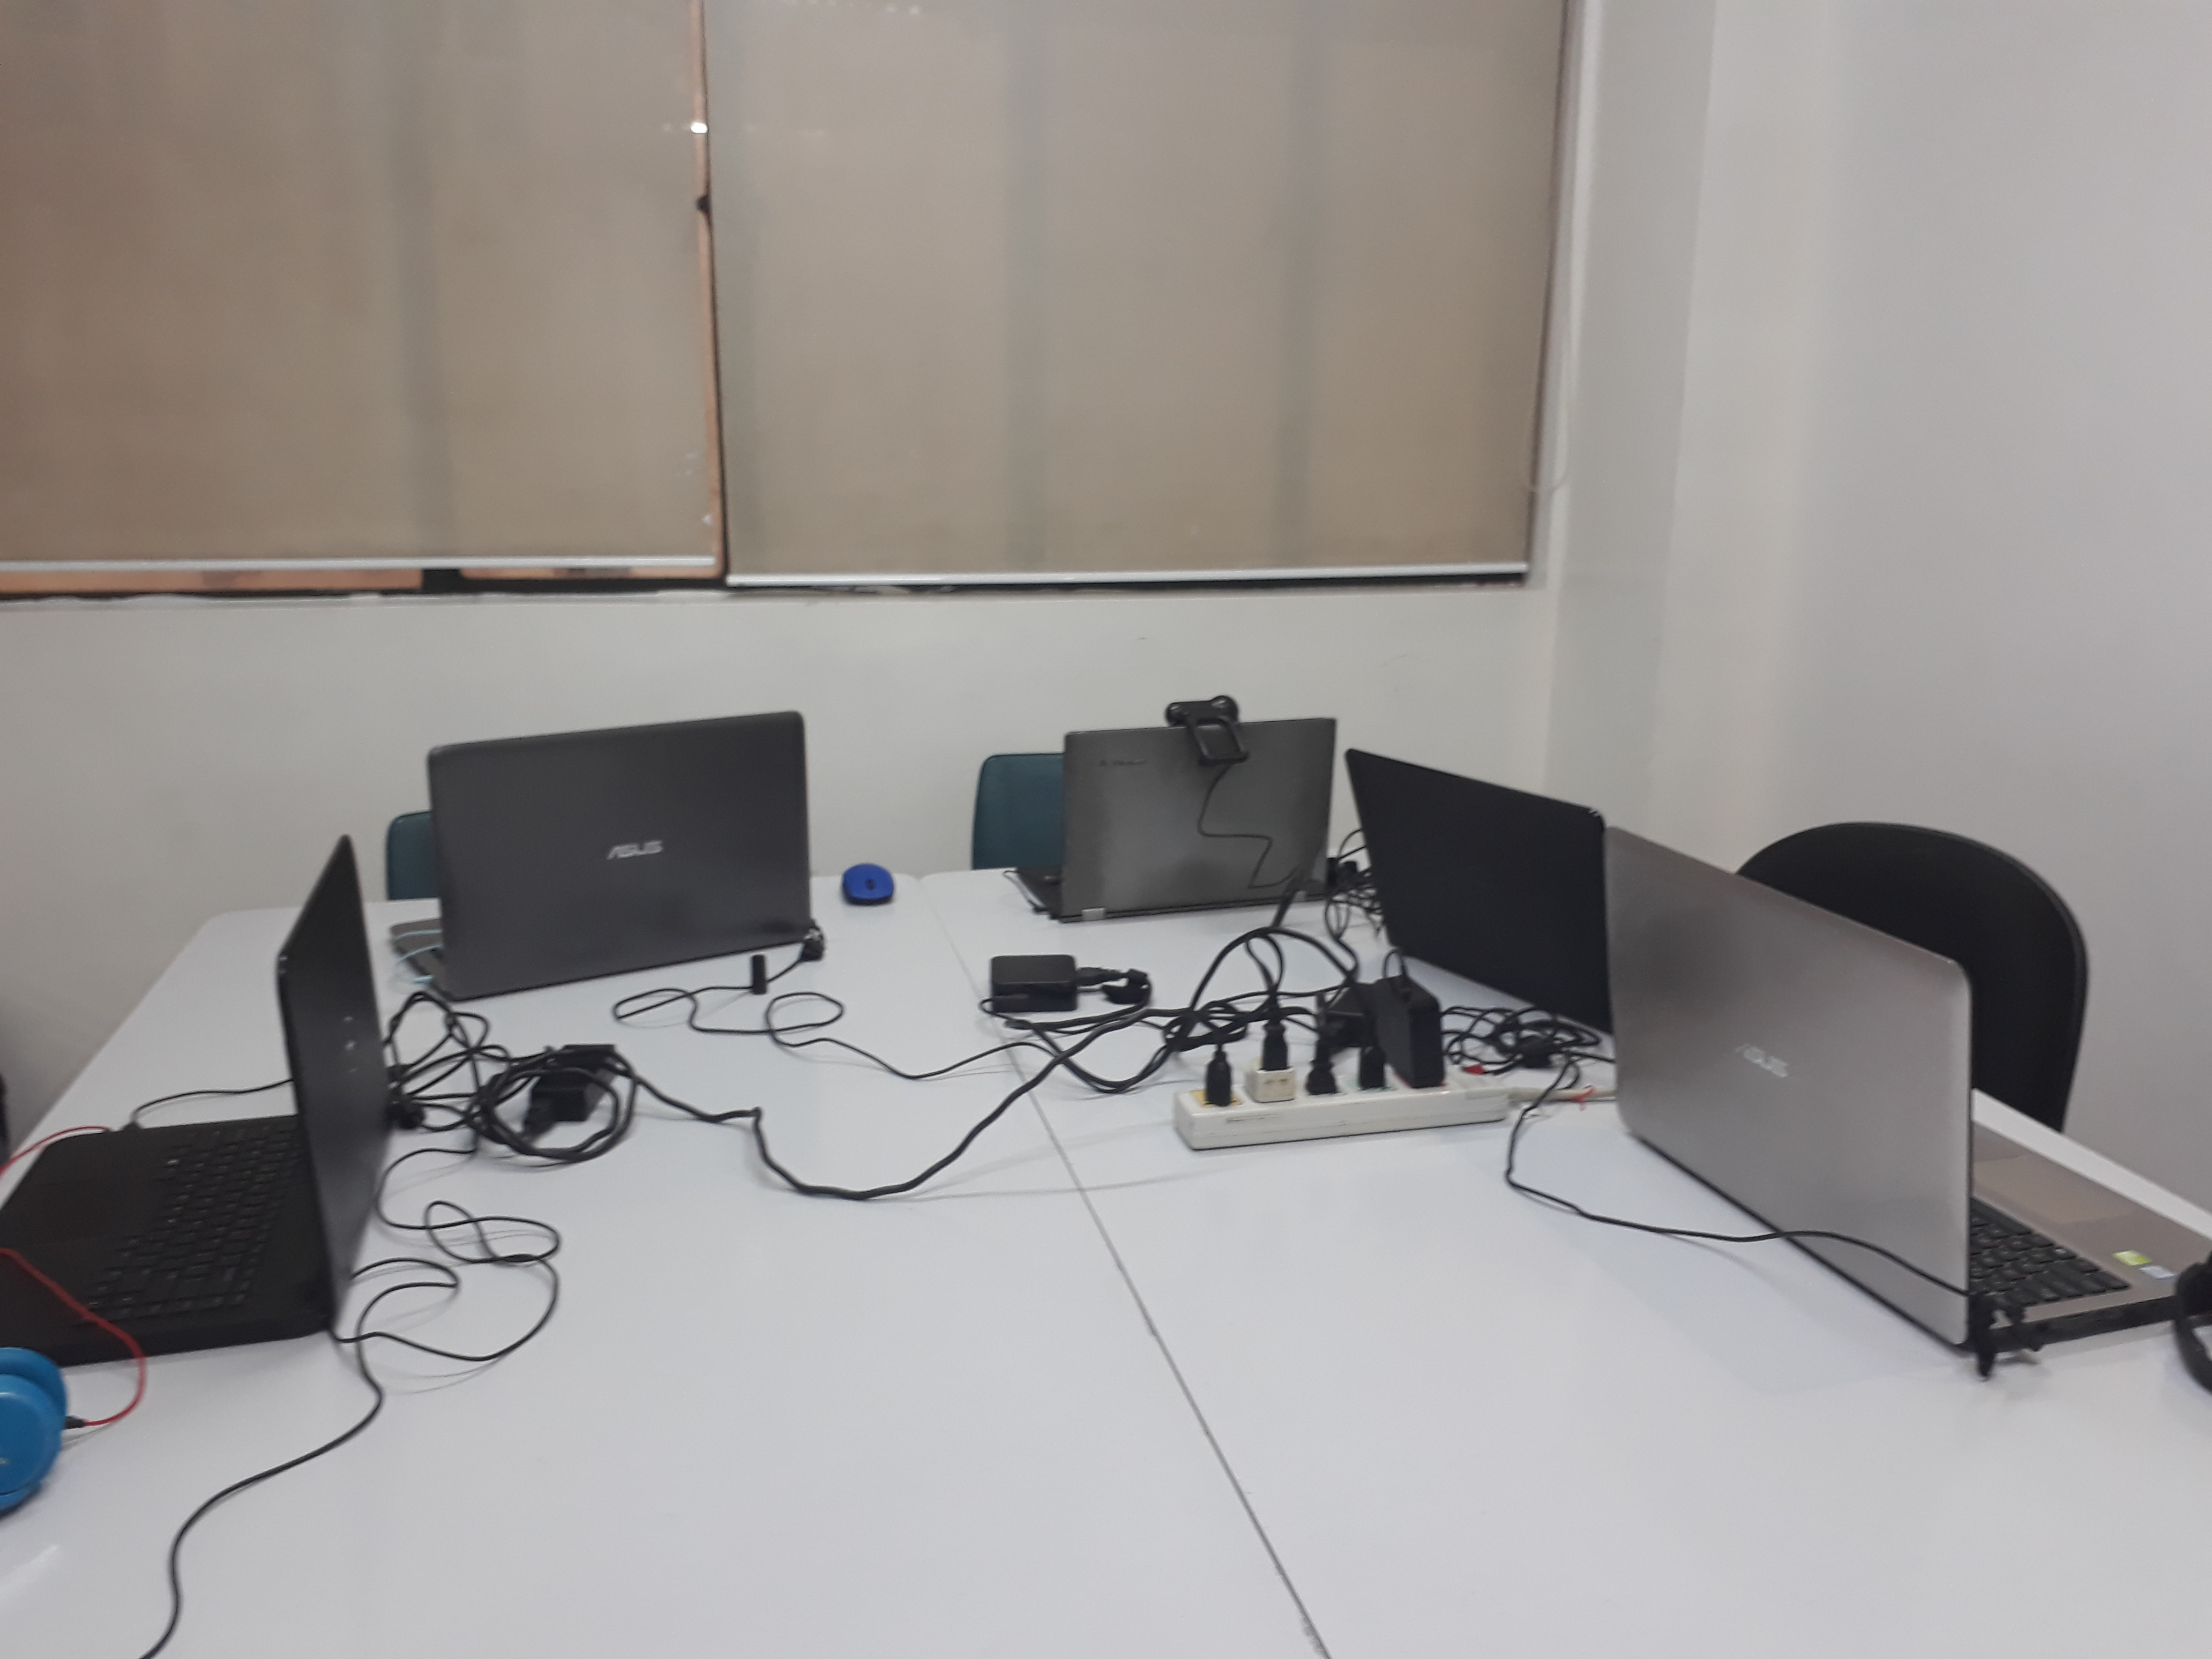
\includegraphics[width=7.5cm,height=4cm]{figures/iter3Setup.jpg}
  \caption{Experiment setup for iteration 3}
  \label{fig:iter3Setup}
\end{figure}
\end{comment}

% Do not change the page size or page settings.
\begin{abstract}
% ViTune aims to enhance the musical experience of the Deaf and Hard of Hearing (DHH) community through the use of an on-screen visualizer generated alongside music. These visualizations were based on related attempts on the visualization of music and were then designed specifically for the DHH community through an iterative testing and feedback process. As of the latest iteration, we were able to identify visual elements which, when seen alongside certain musical elements, resulted in the experience of specific affects. For future work, we plan on adding more features deemed useful by the DHH community, validating the visualizer with an automated testing methodology, comparing the prototype with currently existing music visualizers, and integrating the features of the visualizer into a music player software.
Machine Learning (ML) suites are readily-available for practical use. There are available packaged software and console libraries that can be modified. However, novice programmers avoid these ML suites due to the abstractions with pre-existing tools. Users with limited programming background that know how these models work, struggle with converting them to code for practical use. We iterated on developing a codeblocks tool for linear regression tasks where we did multiple usability tests involving at least 33 participants. We observed how they went through their ML tasks, and inquired into their pains and struggles in writing code. To help them in this learning process, we present TREX: A Toolbox for Regression Experiments, that allows novices in ML programming to gain more confidence with building code. We also derived and verified design guidelines towards providing affordanaces that cater to their needs. 


%Experienced programmers typically follow the Edit-Explore-Guess activity flow. In contrast, we found novices that struggle with code tend to follow Explore-Edit-Guess flow wherein they explore their environment before they gain more confidence with building code. We conclude by deriving design guidelines to provide affordances that cater to their needs.

% In this paper, we present a draft framework and plan that describes the considerations in the creation of a visualization system made for augmenting the musical experience of the Deaf and Hard of Hearing (DHH) community. The goal is to design a system that improves how the DHH currently process input from music through non-auditory means. The development of such system involves careful consideration of the current DHH musical perspectives as well as designing visualization techniques which fulfill such needs. A description of a prototype tool in its early stages, initial user tests along with plans for future work concerning the prototype and the study in general, have been included.
\end{abstract}

\keywords{\plainkeywords}
\begin{CCSXML}
<ccs2012>
<concept>
<concept_id>10003120.10003145.10011770</concept_id>
<concept_desc>Human-centered computing~Visualization design and evaluation methods</concept_desc>
<concept_significance>100</concept_significance>
</concept>
<concept>
<concept_id>10003120.10003121.10003122.10010854</concept_id>
<concept_desc>Human-centered computing~Usability testing</concept_desc>
<concept_significance>500</concept_significance>
</concept>
<concept>
<concept_id>10011007.10011074.10011092.10010876</concept_id>
<concept_desc>Software and its engineering~Software prototyping</concept_desc>
<concept_significance>500</concept_significance>
</concept>
<concept>
<concept_id>10003120.10003121.10003122.10003334</concept_id>
<concept_desc>Human-centered computing~User studies</concept_desc>
<concept_significance>300</concept_significance>
</concept>
</ccs2012>
\end{CCSXML}
% \begin{CCSXML}
% <ccs2012>

% <concept>
% <concept_id>10003120.10003145.10011770</concept_id>
% <concept_desc>Human-centered computing~Visualization design and evaluation methods</concept_desc>
% <concept_significance>500</concept_significance>
% </concept>

% <concept>
% <concept_id>10010405.10010469.10010475</concept_id>
% <concept_desc>Applied computing~Sound and music computing</concept_desc>
% <concept_significance>300</concept_significance>
% </concept>

% <concept>
% <concept_id>10011007.10011074.10011092.10010876</concept_id>
% <concept_desc>Software and its engineering~Software prototyping</concept_desc>
% <concept_significance>100</concept_significance>
% </concept>

% </ccs2012>
% \end{CCSXML}

\ccsdesc[500]{Human-centered computing~Visualization design and evaluation methods}
% \ccsdesc[300]{Applied computing~Sound and music computing}
\ccsdesc[100]{Software and its engineering~Software prototyping}

% Print the classficiation codes
\printccsdesc
% Please use the 2012 Classifiers and see this link to embed them in the text: \url{https://dl.acm.org/ccs/ccs_flat.cfm}

% \marginpar{%
%   \vspace{-45pt} \fbox{%
%     \begin{minipage}{0.925\marginparwidth}
%       \textbf{Good Utilization of the Side Bar} \\
%       \vspace{1pc} \textbf{Preparation:} Do not change the margin
%       dimensions and do not flow the margin text to the
%       next page. \\
%       \vspace{1pc} \textbf{Materials:} The margin box must not intrude
%       or overflow into the header or the footer, or the gutter space
%       between the margin paragraph and the main left column. The text
%       in this text box should remain the same size as the body
%       text. Use the \texttt{{\textbackslash}vspace{}} command to set
%       the margin
%       note's position. \\
%       \vspace{1pc} \textbf{Images \& Figures:} Practically anything
%       can be put in the margin if it fits. Use the
%       \texttt{{\textbackslash}marginparwidth} constant to set the
%       width of the figure, table, minipage, or whatever you are trying
%       to fit in this skinny space.
%     \end{minipage}}\label{sec:sidebar} }

%Codeblocks iterations

%Codeblocks iterations


\section{Introduction}
Off-the-shelf Machine Learning (ML) programs that are ready to use such as WEKA and RapidMiner, were designed to enable novices to conduct experiments without worrying about the code in between. However, this is what some refer to as the blackbox effect, where users do not see the inner workings of a tool. Users who venture into ML experience one of two issues when starting out in the field. They are either (1) computing professionals who have adequate programming experience but may not have the adequate foundation in ML or (2) other professionals who have no adequate programming experience but have preliminary knowledge on activities in the ML pipeline. ML platforms such as WEKA \& Rapidminer fall into the category of tools with a visual interface. 

\begin{marginfigure}[-7.5pc]
\begin{minipage}{\marginparwidth}
     \centering
    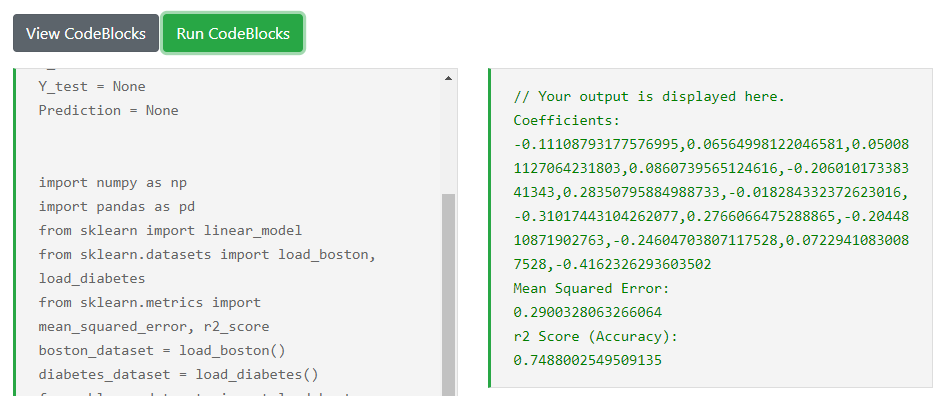
\includegraphics[width=4.5cm,height=2.5cm]{figures/Code_Output.png}
    \caption{Snippet of Code Output and Translation Section}
    \label{fig:Code_output}
    \end{minipage}
\end{marginfigure}

\begin{marginfigure}[1.5pc]
\begin{minipage}{\marginparwidth}
     \centering
    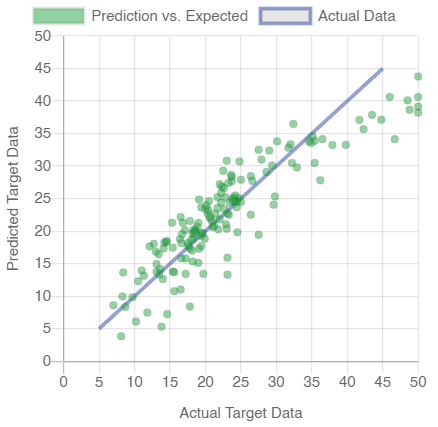
\includegraphics[width=4.5cm,height=4.5cm]{figures/Reg_Vis.png}
    \caption{The Sandbox Prototype Regression Visualization}
    \label{fig:Code_output}
    \end{minipage}
\end{marginfigure}

In the comparison done in the work of \cite{nodalo2019building}, these visual tools are not entirely interactive. They provide limited user feedback and abstracts the algorithm code from the user. One example of an environment with an interactive visualization is TensorFlow Playground \cite{smilkov2017neural}.  TF Playground allows users to tweak with the parameters of a neural network model and then provides visual feedback on a given user-input configuration. Similar to the tools mentioned earlier, the underlying algorithm that runs on its engine are abstracted and hidden away from the regular user of these interfaces. Thus, novice programmers usually encounter difficulty using these tools. A visual interface must be accompanied by design elements that guide the user towards understanding these models and equations. Our works makes an inquiry into the underlying design factors that affect these behaviours. We sought to understand the human factors involving novice users when operating in an unfamiliar, block-based visual interface. We did a formative study composed of interviews, observations, and user tests with 10 participants with varying years of experiences both in programming and ML. We developed a prototype based on their insights which we iteratively tested with 23 more participants. In this paper we: (1) Observe and understand how programmers embark, solve and implement code when given a linear regression task. We also (2) derive and formulate guidelines towards an interactive machine learning (iML) environment prototype that these programmers can use for their regression experiments. Additionally, we (3) discuss design implications for supporting the interaction needs of a novice programmer. Lastly, we (4) Reflect on how we can design better iML platforms that facilitate novice to expert transitions in regression experiments.



\section{Related Work}
There have been studies that have attempted to develop interactive machine learning (iML) environments. In the work of \cite{sarkar2015interactive}, novice ML students are exposed to ML while taking advantage of the interactive environment of standard spreadsheets. These platforms are often limited to their domain, such as finance and economics. Yet, due to the interactive interface of spreadsheets, end-users easily understand how minor tweaking of formulas affect the output of these systems. These systems widen the range of practicality of using ML, allowing to be expanded to other fields. The study of \cite{amershi2012regroup} conducted a research on the use of iML system that classified groups of people on social-networking websites to reduce the instance of unwanted data leaking to people. These systems are able to give end-users an opportunity to work and explore their experiments while considering other specific constraints and ethical considerations. If the need for traditional programming skills to utilize ML algorithms is removed, then the barrier that limits the use of ML in other fields is also reduced. 
% Recent works investigate playfulness and possibilities in various systems \cite{wexler2019if}. They investigate on probing activities of users towards understanding their performance in their tasks. 
The work of \cite{das2019beames, zhao2019featureexplorer} have attempted to design sandbox environments for regression experiments. They consider steering, inspection of ML but do not investigate on the activities and behaviors of the users themselves. TensorFlow is an open source ML framework that deals with high numerical computations \cite{tensorflow_2015}. It is designed to be accessible on different platforms and was created for faster processing of ML algorithms, especially those that can be programmed with Tensors. TensorFlow Playground is an exploratory sandbox that allows users to visualize how a Neural Network learns \cite{tensorflow_2016}. The playground displays various components that the user can tweak which can also affect the output being displayed on the interface.
%Methodology Figure
\begin{marginfigure}[-5.5pc]
\begin{minipage}{\marginparwidth}
     \centering
    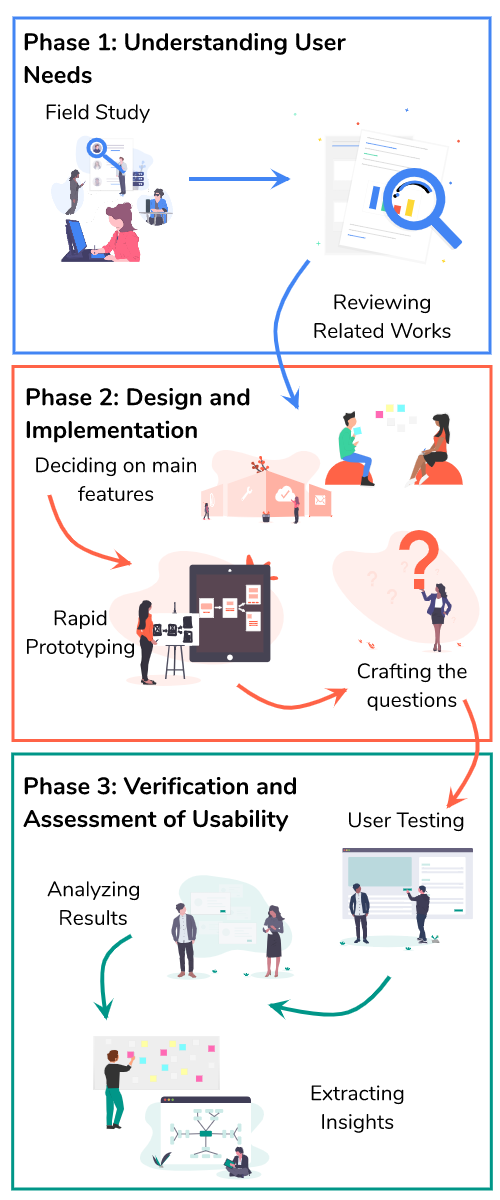
\includegraphics[width=4.5cm,height=12.5cm]{figures/Method-strip.png}
    \caption{Overview of the derived Research Framework, that follows a user-centric, and iterative approach based on the work of \protect\cite{nodalo2019building}. This user-centric approach involves ML novice programmers through each iteration of design and development of the tool.}
    \label{fig:methodology}
    \end{minipage}
\end{marginfigure}
Algorithm Visualization (AV) also plays a role in improving a user's understanding of how an algorithm works \cite{shaffer2010algorithm}. The work of \cite{vrachnos2008dave} had a dynamic AV that exposed novice learners to underlying algorithm logic. Platforms like this help fit the mental model of the user and their perceptions about the behavior of the algorithm itself. There are also AV platforms that considered the relevance of the learning algorithms as they grew with the demand for better visualizations. Learning algorithms have been made unified and interactive on web-based platforms which is seen in the work of \cite{halim2012learning}. These improved the way novice learners absorbed lessons on algorithms with the help of appropriate scripted examples and animations. However, it is focused on visualizing data structures and non-ML algorithms. Designing for effective end-user interaction with ML systems attempted to define a set of design factors that would govern the design considerations for creating an effective iML system \cite{amershi2011designing}. They considered several design factors such as Interaction Focus, Intended Product, Evolutionary Needs, Concept Flexibility, Performance Requirements and Model Ownership. These helped the research in understanding users of iML systems involving other approaches. Exploring user-centered design with methods such as Agile methods in software design may sometimes cause conflict in developing user-centered iML tools due to the lack of usability awareness in its process \cite{da2011user}. It has been observed that the programmers in agile settings consider factors that give them flexibility instead \cite{hussain2009current}. However, the study of \cite{sarkar2015interactive} observed users that often preferred a specific user flow as a result of using these iML systems, which were discovered from applying user-centered design process in an agile setting. Ideally, this approach involving end-user innovation on iML systems states that the user centered design process can be applied to improve usability itself for novice users \cite{bernardo2016interactive} and systems targeted for their use. Several works have investigated on behaviors and productivity of programmers coming from different backgrounds and experiences. In this research, we look at how these works can be pushed forward towards understanding design guidelines, building a tool considering these guidelines and investigating how these guidelines can possibly help novice programmers especially in doing machine learning tasks. 
\section{Methodology}
For this study, the methodology follows three (3) main phases as seen in figure \ref{fig:methodology}. The framework used for the methodology is continuation of a previous study by \cite{nodalo2019building} which follows an iterative approach. In relation to this study, it involves designing and testing multiple version of the Regression tool to improve previous iterations. A total of three (3) iterations were completed throughout the study accompanied by prior user research to aid with forming the features and interactions to address painpoints mentioned by potential novice users. All iterations were tested by undergraduate and graduate students that have a basic background of programming and ML. 
\subsection{User Research}
Prior to prototyping the Regression Tool, an initial user study was conducted through in-depth interviews with undergraduate and graduate students with a computing background. These students are programmers with familiarity of ML, especially with programming Linear Regression. We refer to them as novice ML programmers. The participants were interviewed about their familiarity with ML concepts and the pain points they encounter while learning and using ML applications and libraries. The concept of code abstractions and code-blocks was briefly discussed with them to gain further insight of their expectations of the Regression tool. 

\begin{marginfigure}[-0.5pc]
\begin{minipage}{\marginparwidth}
     \centering
    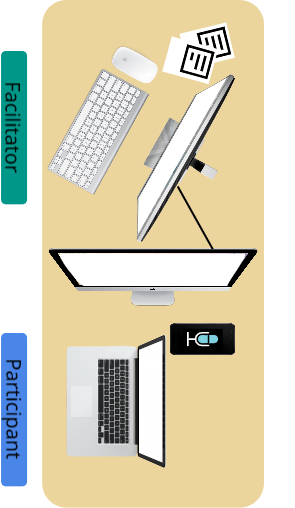
\includegraphics[width=4.5cm,height=7cm]{figures/setup.png}
    \caption{Test Setup for all usability testing of prototypes.}
    \label{fig:setup}
    \end{minipage}
\end{marginfigure}
\begin{marginfigure}[1.5pc]
\begin{minipage}{\marginparwidth}
     \centering
    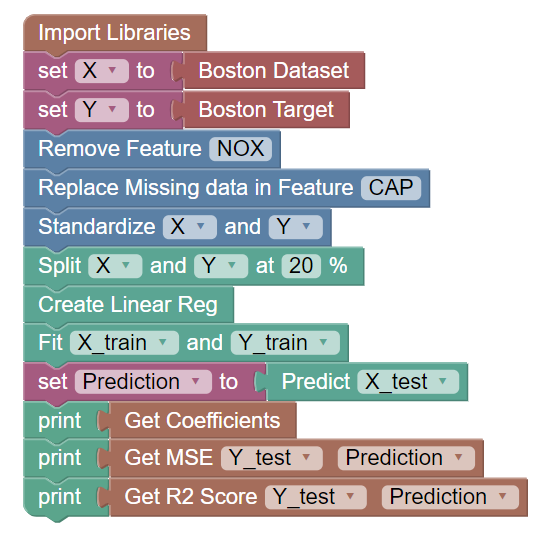
\includegraphics[width=4.5cm,height=4.5cm]{figures/IT2.png}
    \caption{Iteration 2 Code Blocks. As compared to Iteration 3 blocks, colors are not organized and sub parameters appear to be confusing.}
    \label{fig:IT2_Blocks}
    \end{minipage}
\end{marginfigure}
\subsection{Iterative Prototyping With Code-block Abstractions}
To design the prototype, insights gathered from the prior user research were used to form user stories that were later converted into features for the tool. Following the interface structure of Scratch developed by \cite{mit:Scratch}, the tool was designed to have three sections in mind \textemdash the code block work space, the code display, and a graph to help visualize the linear regression model created. Initially, a prototype using static code blocks that followed similar naming conventions to Scikit Learn's Linear Regression library was developed and tested in each iteration. Each category of code blocks were assigned specific colors to represent the phases of the ML pipeline. For the static prototype, three code block categories were prepared \textemdash Data Preprocessing, Linear Regression, and Test Model. An interactive prototype was later developed. We used Google Blockly (the same code block technology used for Scratch), as the main interfacing blocks for the tool. The Scikit Learn Linear Regression library functions were used for creating the Linear Regression model. To support its functions, Python's Django web framework allowed the tool to run Python code generated from the code blocks. The generated code is then executed by the Python compiler. In addition, Chart.js aided with creating the Linear Regression visualization by providing an interactive scatter plot that updates as the model is updated. Due to certain limitations with the libraries used, three additional code block categories were added to the iML prototype. These being Libraries used for importing the necessary Python libraries required for the Linear Regression model, Variables which contain code blocks of predefined variables created for the iML tool, and Dataset for importing the online datasets recommended for use by Scikit Learn. 

\subsection{Usability Testing Codeblock Environment}
The prototypes were iteratively tested through usability testing. The first iteration tested the static code blocks provided using a prototyping tool. Each participant was tasked to map code blocks based on their understanding of the two Linear Regression two code samples provided. The second and third iteration were done and tested using the main code environment of the tool. The second iteration served as the initial interactive version of the iML tool. This version had no graphical visualization of the Linear Regression model but had the other basic features working. Some insights from the first iteration were used to improve the code block design implemented for the second iteration. Participants were tasked to create Linear Regression systems with the two datasets used for the tool. The second iteration focused on discoverability. We did this to observe user activity flows and determine the common interactions participants would follow when using the code blocks and when exposed to familiar programming environments such as using Google's Collaboratory. Using suggestions for improvement from the second iteration, the third iteration prototype was developed and tested following a similar approach to the previous iteration. Four (4) tasks were given to the testers to exhaustively explore the tool's features. Additionally, a graphical visualization of the model was added in this version to visualize the generated predictions of the model. The focus of this iteration is to test the specific features of the iML tool and to observe how additional visualization of the model would influence how users would create Linear Regression systems. 

\subsection{Test Design and Experiment Setup}
The experiment setup for each iteration can be seen in figure \ref{fig:setup}. This setup remained consistent for both the static (first iteration) and interactive (second and third iteration) prototypes tested. The Participant was positioned in front of a laptop with the prototype available. The Facilitator was positioned beside the participant while tracking screen movement was tracked and recorded from the external monitor. The web camera of the desktop computer between the external monitor and the laptop was used to record the participants reactions and displayed the test flow and tasks. A voice recorder was used to record extra audio for the test. After each test, post-test surveys such as the System Usability Scale (SUS) survey and a Guidelines Heuristic Review survey were issued before conducting a short post-test interview to understand the participant's experience using the prototype. 

 \begin{margintable}[-23.5pc]
   \begin{minipage}{\marginparwidth}
     \centering
     \begin{tabular}{@{}cr@{}}
       \multicolumn{2}{r}{\textbf{Average Score for Iteration 2}} \\
       \midrule
       \textbf{Participant} & \multicolumn{1}{c}{\textbf{SUS Score}} \\ \midrule
        1 & 57.50 \\
        2 & 77.50 \\
        3 & 37.50 \\
        4 & 72.50 \\
        5 & 92.50 \\
        6 & 47.50 \\
        7 & 72.50 \\
        8 & 45.00 \\
        9 & 67.50 \\
        10 & 60.00 \\
        \begin{tabular}[c]{@{}c@{}}Average\end{tabular} & 63.00 \\
       \bottomrule
     \end{tabular}
     \caption{Average survey score for iteration 2 of the iML tool}
     \label{tab:it2_sus}
   \end{minipage}
 \end{margintable}
 
  \begin{margintable}[-2.5pc]
   \begin{minipage}{\marginparwidth}
     \centering
     \begin{tabular}{@{}cr@{}}
    \multicolumn{2}{r}{\textbf{SUS Score for Iteration 3}} \\ \midrule
    \textbf{Participant} & \multicolumn{1}{c}{\textbf{SUS Score}} \\ \midrule
    1 & 85.00 \\
    2 & 85.00 \\
    3 & 85.00 \\
    4 & 72.50 \\
    5 & 75.00 \\
    \begin{tabular}[c]{@{}c@{}}Average\end{tabular} & 80.50 \\ \bottomrule
    \end{tabular}
     \caption{Average survey score for iteration 3 of the iML tool}
     \label{tab:it3_sus}
   \end{minipage}
 \end{margintable}


\section{Results}

\subsection{Iteration Testing}
Each of the three (3) iterations of the prototype was tested by at least five (5) ML users with varying skill levels, where two (2) of which identified themselves as novice users. For iteration 1, all novice users were intuitively trying to follow a pattern based on the ML Pipeline: Data Preprocessing, Model Training, and Model Testing. These users were also consistent when ordering the Fit Data and Predict blocks. They placed the create-model block outside the model bracket. Novice users were observed to be experimental and contemplating using data preprocessing and testing blocks. These users found the tasks manageable. They also noted that organizing different ML phases by color made it easier, but were confused with the blocks for data preprocessing. For iteration 2, ten (10) ML users were recruited using purposive sampling. Most users enjoying the satisfying sounds the system makes when connecting blocks which reassures them of their progress. They also cited how the order of the blocks and categories are ordered to follow the ML pipeline they identified. However, some users found it intimidating and stressful with some users skipping some of the tasks due to misunderstanding the purpose of the tool, such as stacking blocks horizontally rather than a top-down approach. They also struggled when figuring out the purpose of the ``Prediction'' block due to the colour of the block and Print block being similar as seen in figure \ref{fig:IT2_Blocks}. Some users felt that the tool limited flexibility when it came to printing outputs, and creating and renaming variables while some users wanted line numbers with proper error messages in the output section similar to traditional IDE's. The SUS survey score from this iteration received an average score of 63.00 which falls into a Grade D - Poor, seen in table \ref{tab:it2_sus}. This means the tool failed in terms of usability as a system. This may be due to the types of errors participants encountered while using the tool and their time adjusting and exploring the code blocks. 

For iteration 3, three (3) ML users were selected for a beta version and another five (5) users were selected for the final version of the prototype, again using purposive sampling. The beta version differs significantly with some of the colors, code block shapes, and error handling compared to the final version which was necessary as some errors were not fully resolved before moving to the final iteration. Most users enjoyed using TREX code blocks to make base linear regression code and motivating to use due to its intuitiveness. However, some participants thought it was vague and a  frustrating to use because they do not understand what some error messages are suggesting for them to do, which often leads to confusion. Due to the previous pain point of connecting the ``Prediction'' block to the ``Print'' block, this lead to the design decision of hard-coding the initialization of the Prediction variable instead of maintaining the male jigsaw green block shape that is similar in color to the native print block. The testing blocks for the final version of the prototype, as seen in figure \ref{fig:IT3_Blocks}, were also recoloured to green to be automatically associate them as output value blocks. The SUS survery score from this iteration received an average score of 80.50 which falls into a Grade A - Excellent, seen in table \ref{tab:it3_sus}. This means the tool is usable and functions towards user expectations. Between Iteration 2 and 3, there clearly is a significant increase in the SUS score from 63 to 80.50.

\subsection{Design Guidelines Review}
In iteration 3, a Guideline Heuristics Review was added to the testing in order to evaluate how well the tool complied with the guideline. The guidelines were formulated by \cite{nodalo2019building} and can be seen in table.  Figure \ref{fig:guidelines} shows a radar graph of the guidelines review results. The closer the web is towards the outer circle, the more the guideline was adhered to by the tool. Thus, the current iML tool created mostly adhered to guidelines 1-4 related to system interaction and visualization. Guideline 5 had mixed results from the iteration 3 participants as some participants are still looking for more descriptive errors. 

%Codeblocks iterations
% \begin{marginfigure}[-17.5pc]
% \begin{minipage}{\marginparwidth}
%      \centering
%     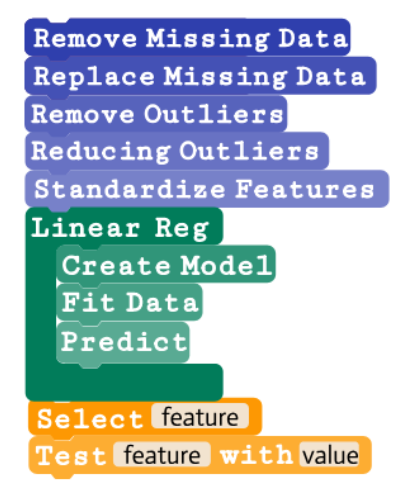
\includegraphics[width=4.5cm,height=4.5cm]{figures/IT1.png}
%     \caption{Iteration 1 Code Blocks}
%     \label{fig:IT1_Blocks}
%     \end{minipage}
% \end{marginfigure}

\begin{marginfigure}[-20.5pc]
\begin{minipage}{\marginparwidth}
     \centering
    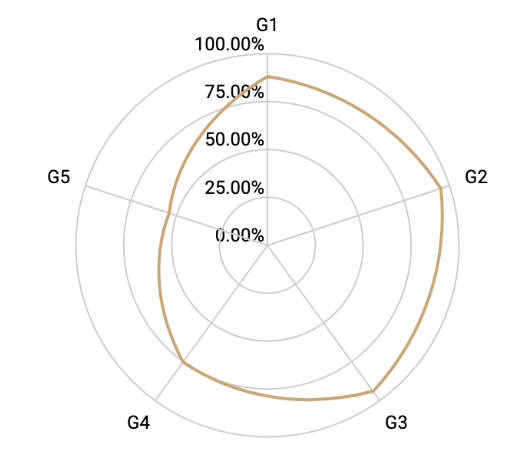
\includegraphics[width=4.5cm,height=4.5cm]{figures/guidelinereview.png}
    \caption{Radar Graph of Heuristic Review on Guidelines. The guidelines derived from \protect \cite{nodalo2019building} are:
    \newline G1 \textemdash The system should indicate to the user its state of change with every interaction.
    \newline G2 \textemdash The components of the interface should be laid out in an organized manner and should be explicitly labelled.
    \newline G3 \textemdash Visualizations should be simple enough to understand and they should not overload the user.
    \newline G4 \textemdash The intent of the system should be clear to the user upon interaction.
    \newline G5 \textemdash The system should indicate explicitly when and why errors occur and how users can recover from them.}
    \label{fig:guidelines}
    \end{minipage}
\end{marginfigure}

\section{Conclusion and Future Work}
As iML platforms are becoming more in demand, it is important to understand the human factors that influence the design of these systems. We designed and developed TREX: A Toolbox for Regression Experiments following the design guidelines that we derived from \cite{nodalo2019building}. Through iterative prototyping and testing, we echo the findings of \cite{sarkar2015interactive} and confirm the guidelines we derived based on \cite{amershi2011designing}. Novice programmers tend to be less confident than their experienced counterparts. The behaviour they exhibited included: (1) exploring first their environment before building their solution as seen from our regression experiments. We then validated our guidelines through a heuristic review and software usability scores. But with limited participants, our findings are yet to be verified through extensive testing. These findings emphasize the dynamic demand for better design in iML systems. With further research, we can still investigate and validate whether these behaviours are observable as well in other ML activities beyond regression experiments. 

\section{Authors}
Jordan Aiko Deja is faculty in the Software Technology Department, College of Computer Studies of De La Salle University, Manila, Philippines. He is also a PhD student at the University of Primorska, Koper, Slovenia. 

Giselle Nodalo and Jose Maria Santiago III  are graduates of De La Salle University Manila, with a Bachelor's Degree in Computer Science - with specialization in Software Technology at De La Salle University Manila, Philippines.

\bibliographystyle{SIGCHI-Reference-Format}
\bibliography{myreferences}
\end{document}
    
% --------------------- v --- Template stuff --- v ----------------------------

% \section{Introduction}

% \section{ACM Copyrights \& Permission Policy}

% \section{Page Size}


% \section{Text Formatting}
% Please use an 8.5-point Verdana font, or other sans serifs font as
% close as possible in appearance to Verdana in which these guidelines
% have been set. Arial 9-point font is a reasonable substitute for
% Verdana as it has a similar x-height. Please use serif or
% non-proportional fonts only for special purposes, such as
% distinguishing \texttt{source code} text.

% \subsubsection{Text styles}
% The \LaTeX\ template facilitates text formatting for normal (for body
% text); heading 1, heading 2, heading 3; bullet list; numbered list;
% caption; annotation (for notes in the narrow left margin); and
% references (for bibliographic entries). Additionally, here is an
% example of footnoted\footnote{Use footnotes sparingly, if at all.}
% text. As stated in the footnote, footnotes should rarely be used.

% \begin{figure}
%   
\includegraphics[width=0.9\columnwidth]{figures/sigchi-logo}
%   \caption{Insert a caption below each figure.}~\label{fig:sample}
% \end{figure}

% \subsection{Language, style, and content}
% The written and spoken language of SIGCHI is English. Spelling and
% punctuation may use any dialect of English (e.g., British, Canadian,
% US, etc.) provided this is done consistently. Hyphenation is
% optional. To ensure suitability for an international audience, please
% pay attention to the following:

% \begin{table}
%   \centering
%   \begin{tabular}{l r r r}
%     % \toprule
%     & & \multicolumn{2}{c}{\small{\textbf{Test Conditions}}} \\
%     \cmidrule(r){3-4}
%     {\small\textit{Name}}
%     & {\small \textit{First}}
%       & {\small \textit{Second}}
%     & {\small \textit{Final}} \\
%     \midrule
%     Marsden & 223.0 & 44 & 432,321 \\
%     Nass & 22.2 & 16 & 234,333 \\
%     Borriello & 22.9 & 11 & 93,123 \\
%     Karat & 34.9 & 2200 & 103,322 \\
%     % \bottomrule
%   \end{tabular}
%   \caption{Table captions should be placed below the table. We
%     recommend table lines be 1 point, 25\% black. Minimize use of
%     table grid lines.}~\label{tab:table1}
% \end{table}

% \begin{itemize}\compresslist%
% \item Write in a straightforward style. Use simple sentence
%   structure. Try to avoid long sentences and complex sentence
%   structures. Use semicolons carefully.
% \item Use common and basic vocabulary (e.g., use the word ``unusual''
%   rather than the word ``arcane'').
% \item Briefly define or explain all technical terms. The terminology
%   common to your practice/discipline may be different in other design
%   practices/disciplines.
% \item Spell out all acronyms the first time they are used in your
%   text. For example, ``World Wide Web (WWW)''.
% \item Explain local references (e.g., not everyone knows all city
%   names in a particular country).
% \item Explain ``insider'' comments. Ensure that your whole audience
%   understands any reference whose meaning you do not describe (e.g.,
%   do not assume that everyone has used a Macintosh or a particular
%   application).
% \item Explain colloquial language and puns. Understanding phrases like
%   ``red herring'' requires a cultural knowledge of English. Humor and
%   irony are difficult to translate.
% \item Use unambiguous forms for culturally localized concepts, such as
%   times, dates, currencies, and numbers (e.g., ``1-5- 97'' or
%   ``5/1/97'' may mean 5 January or 1 May, and ``seven o'clock'' may
%   mean 7:00 am or 19:00). For currencies, indicate equivalences:
%   ``Participants were paid {\fontfamily{txr}\selectfont \textwon}
%   25,000, or roughly US \$22.''
% \item Be careful with the use of gender-specific pronouns (he, she)
%   and other gender-specific words (chairman, manpower,
%   man-months). Use inclusive language (e.g., she or he, they, chair,
%   staff, staff-hours, person-years) that is gender-neutral. If
%   necessary, you may be able to use ``he'' and ``she'' in alternating
%   sentences, so that the two genders occur equally
%   often~\cite{Schwartz:1995:GBF}.
% \item If possible, use the full (extended) alphabetic character set
%   for names of persons, institutions, and places (e.g.,
%   Gr{\o}nb{\ae}k, Lafreni\'ere, S\'anchez, Nguy{\~{\^{e}}}n,
%   Universit{\"a}t, Wei{\ss}enbach, Z{\"u}llighoven, \r{A}rhus, etc.).
%   These characters are already included in most versions and variants
%   of Times, Helvetica, and Arial fonts.
% \end{itemize}

% % \begin{figure}
% %   \includegraphics[width=.9\columnwidth]{figures/ea-figure2}
% %   \caption{If your figure has a light background, you can set its
% %     outline to light gray, like this, to make a box around
% %     it.}\label{fig:bats}
% % \end{figure}

% \begin{marginfigure}[-35pc]
%   \begin{minipage}{\marginparwidth}
%     \centering
%     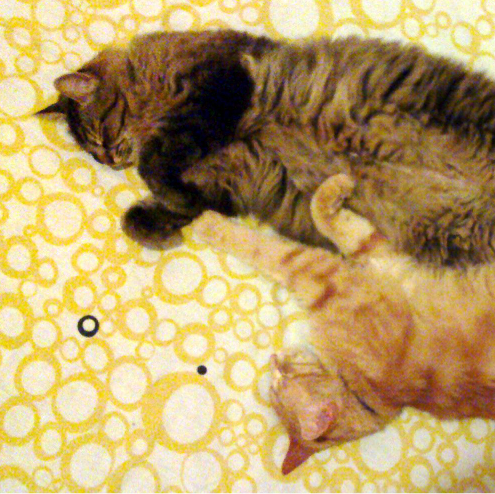
\includegraphics[width=0.9\marginparwidth]{figures/cats}
%     \caption{In this image, the cats are tessellated within a square
%       frame. Images should also have captions and be within the
%       boundaries of the sidebar on page~\pageref{sec:sidebar}. Photo:
%       \cczero~jofish on Flickr.}~\label{fig:marginfig}
%   \end{minipage}
% \end{marginfigure}

% \section{Figures}
% The examples on this and following pages should help you get a feel
% for how screen-shots and other figures should be placed in the
% template. Your document may use color figures (see
% Figures~\ref{fig:sample}), which are included in the page limit; the
% figures must be usable when printed in black and white. You can use
% the \texttt{\marginpar} command to insert figures in the (left) margin
% of the document (see Figure~\ref{fig:marginfig}). Finally, be sure to
% make images large enough so the important details are legible and
% clear (see Figure~\ref{fig:cats}).
% All figures should include alt text (figure description) for improved accessibility – see the Accessibility section.

% \section{Tables}
% You man use tables inline with the text (see Table~\ref{tab:table1})
% or within the margin as shown in Table~\ref{tab:table2}. Try to
% minimize the use of lines (especially vertical lines). \LaTeX\ will
% set the table font and captions sizes correctly; the latter must
% remain unchanged.

% \section{Accessibility}
% The Executive Council of SIGCHI has committed to making SIGCHI
% conferences more inclusive for researchers, practitioners, and
% educators with disabilities. As a part of this goal, the all authors
% are expected to work on improving the accessibility of their
% submissions. Specifically, we encourage authors to carry out the
% following five steps:
% \begin{itemize}\compresslist%
% \item Add alternative text (figure description) to all figures
% \item Mark table headings
% \item Generate a tagged PDF
% \item Verify the default language
% \item Set the tab order to ``Use Document Structure''
% \end{itemize}

% For links to detailed instructions and resources, please see:
% \url{http://chi2020.acm.org/authors/papers/guide-to-an-accessible-submission/}

% Unfortunately good tools do not yet exist to create tagged PDF files
% from Latex. \LaTeX\ users will need to carry out all of the above
% steps in the PDF directly using Adobe Acrobat, after the PDF has been
% generated.


% \begin{figure*}
%   \centering
%   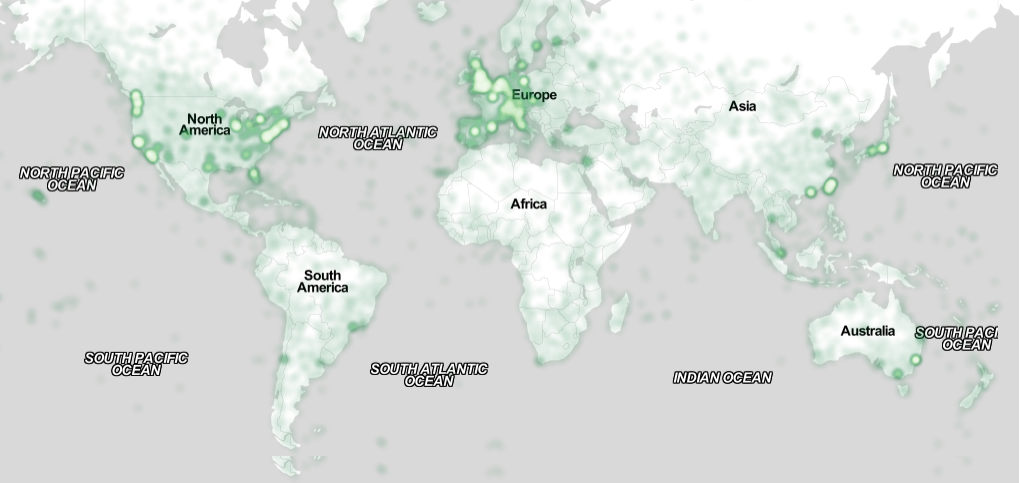
\includegraphics[width=1.3\columnwidth]{figures/map}
%   \caption{In this image, the map maximizes use of space. You can make
%     figures as wide as you need, up to a maximum of the full width of
%     both columns. Note that \LaTeX\ tends to render large figures on a
%     dedicated page. Image: \ccbynd~ayman on Flickr.}~\label{fig:cats}
% \end{figure*}

% \section{Producing and Testing PDF Files}
% We recommend that you produce a PDF version of your submission well
% before the final deadline. Your PDF file must be ACM DL Compliant and
% meet stated requirements,
% \url{http://www.sheridanprinting.com/sigchi/ACM-SIG-distilling-settings.htm}.

% \marginpar{\vspace{-23pc}So long as you don't type outside the right
%   margin or bleed into the gutter, it's okay to put annotations over
%   here on the left, too; this annotation is near Hawaii. You'll have
%   to manually align the margin paragraphs to your \LaTeX\ floats using
%   the \texttt{{\textbackslash}vspace{}} command.}


% Test your PDF file by viewing or printing it with the same software we
% will use when we receive it, Adobe Acrobat Reader Version 10. This is
% widely available at no cost. Note that most
% reviewers will use a North American/European version of Acrobat
% reader, so please check your PDF accordingly.

% \section{Acknowledgements}
% We thank all the volunteers, publications support, staff, and authors
% who wrote and provided helpful comments on previous versions of this
% document. As well authors 1, 2, and 3 gratefully acknowledge the grant
% from NSF (\#1234--2222--ABC). Author 4 for example may want to
% acknowledge a supervisor/manager from their original employer. This
% whole paragraph is just for example. Some of the references cited in
% this paper are included for illustrative purposes only.

% \section{References Format}
% Your references should be published materials accessible to the
% public. Internal technical reports may be cited only if they are
% easily accessible and may be obtained by any reader for a nominal
% fee. Proprietary information may not be cited. Private communications
% should be acknowledged in the main text, not referenced (e.g.,
% [Golovchinsky, personal communication]). References must be the same
% font size as other body text. References should be in alphabetical
% order by last name of first author. Use a numbered list of references
% at the end of the article, ordered alphabetically by last name of
% first author, and referenced by numbers in brackets. For papers from
% conference proceedings, include the title of the paper and the name of
% the conference. Do not include the location of the conference or the
% exact date; do include the page numbers if available. 

% References should be in ACM citation format:
% \url{http://www.acm.org/publications/submissions/latex_style}.  This
% includes citations to Internet
% resources~\cite{CHINOSAUR:venue,cavender:writing,psy:gangnam}
% according to ACM format, although it is often appropriate to include
% URLs directly in the text, as above. Example reference formatting for
% individual journal articles~\cite{ethics}, articles in conference
% proceedings~\cite{Klemmer:2002:WSC:503376.503378},
% books~\cite{Schwartz:1995:GBF}, theses~\cite{sutherland:sketchpad},
% book chapters~\cite{winner:politics}, an entire journal
% issue~\cite{kaye:puc},
% websites~\cite{acm_categories,cavender:writing},
% tweets~\cite{CHINOSAUR:venue}, patents~\cite{heilig:sensorama}, 
% games~\cite{supermetroid:snes}, and
% online videos~\cite{psy:gangnam} is given here.  See the examples of
% citations at the end of this document and in the accompanying
% \texttt{BibTeX} document. This formatting is a edited version of the
% format automatically generated by the ACM Digital Library
% (\url{http://dl.acm.org}) as ``ACM Ref''. DOI and/or URL links are
% optional but encouraged as are full first names. Note that the
% Hyperlink style used throughout this document uses blue links;
% however, URLs in the references section may optionally appear in
% black.

\balance{} 

\bibliographystyle{SIGCHI-Reference-Format}
\bibliography{sample}

\end{document}

%%% Local Variables:
%%% mode: latex
%%% TeX-master: t
%%% End:
